\documentclass[conference]{IEEEtran}
\usepackage[utf8]{inputenc}
\usepackage[T1]{fontenc}
\usepackage{amsmath,amssymb}
\usepackage{graphicx}
\usepackage{booktabs}
\usepackage{tikz}
\usetikzlibrary{positioning,arrows.meta}
\usepackage{cite}
\usepackage{array}
\usepackage{enumitem}

% numbers filled in by ML/results_to_latex.py (see results_macros.tex)
\newcommand{\hybErr}{}\newcommand{\hybFscore}{}\newcommand{\hybPrec}{}\newcommand{\hybRec}{}\newcommand{\hybAcc}{}
\newcommand{\bestBaseName}{}\newcommand{\bestBaseErr}{}\newcommand{\relRedBase}{}\newcommand{\paperErr}{}\newcommand{\relRedPaper}{}
% Placeholder values. Overwritten by: python ML/results_to_latex.py --dataset cicids2017 --paper-error <x> --out Documentation/Paper
\renewcommand{\hybErr}{[run results\_to\_latex.py]}
\renewcommand{\hybFscore}{[run]}
\renewcommand{\hybPrec}{[run]}
\renewcommand{\hybRec}{[run]}
\renewcommand{\hybAcc}{[run]}
\renewcommand{\bestBaseName}{[run]}
\renewcommand{\bestBaseErr}{[run]}
\renewcommand{\relRedBase}{[run]}
\renewcommand{\paperErr}{[run]}
\renewcommand{\relRedPaper}{[run]}


\begin{document}

\title{Zero-Day Attack Framework Using Machine Learning-Based Anomaly Detection}

\author{\IEEEauthorblockN{Author One, Author Two, Author Three, Author Four}
\IEEEauthorblockA{Department of Computer Science and Engineering\\
Mohan Babu University, India\\
\{email1, email2, email3, email4\}@example.edu}}

\maketitle

\begin{abstract}
Signature-based intrusion detection cannot recognise attacks it has never seen, and labelled data for novel attacks does not exist by definition. This work presents a practical framework for flagging zero-day network traffic by combining an unsupervised anomaly detector with a supervised classifier. An Isolation Forest, fitted only on benign flows, produces a calibrated anomaly percentile; this percentile is appended to the flow features and passed to a gradient-boosted tree classifier trained on SMOTE-balanced data. The two outputs are blended with a weight and a decision threshold that are tuned on a validation set containing an attack family withheld from training, and the blended score is mapped to a 0--100 risk score with severity bands. We evaluate with a leave-one-attack-family-out protocol on CIC-IDS2017 and compare six models on accuracy, precision, recall, F1-score and error rate. The proposed hybrid reaches an error rate of \hybErr{} and an F1-score of \hybFscore{}; the best single baseline (\bestBaseName) reaches \bestBaseErr{}. The detector is deployed behind a REST service and a web dashboard so analysts can upload flow files, review alerts and export reports.
\end{abstract}

\begin{IEEEkeywords}
zero-day attack, anomaly detection, intrusion detection, Isolation Forest, XGBoost, ensemble learning, CIC-IDS2017
\end{IEEEkeywords}

\section{Introduction}
Network defenders increasingly face attacks for which no signature, rule or labelled training example exists. Classifiers trained on known attack classes tend to score unfamiliar traffic as benign, because the decision boundary was never shaped by that behaviour. Anomaly detectors take the opposite view: they model normal traffic and treat large deviations as suspicious, which allows novel attacks to be caught but at the price of false alarms on legitimate but unusual traffic \cite{chandola2009anomaly}.

Recent work has pursued representation learning on traffic graphs to score unseen malicious flows \cite{basepaper2026}. Such approaches are powerful but depend on graph construction and self-supervised pre-training that are heavy to reproduce and to operate. Our goal is more modest and operational: a framework built from well-understood components that a small security team could train on its own flow logs, evaluate honestly against unseen attack families, and run behind a web interface.

The contributions of this paper are:
\begin{itemize}
\item A hybrid scoring model that feeds a calibrated Isolation Forest percentile into a gradient-boosted classifier and blends both outputs, with the blend weight and threshold tuned on a pseudo-unknown attack family.
\item A strict leave-one-attack-family-out evaluation in which every model, including the unsupervised ones, receives a threshold tuned on the same validation data.
\item A risk-scoring layer that converts model scores into a 0--100 value, a severity level and a threat type (known attack, suspected zero-day, or suspicious anomaly).
\item An end-to-end system: a Python inference service, an ASP.NET Core API with role-based access and auditing, and an MVC dashboard.
\end{itemize}

\textbf{Problem statement.} Given a stream of network flows in which some attack behaviours have never been labelled, flag the flows that deserve analyst attention, rank them by risk, and do so with a false-alarm rate low enough for an operations team to use. The objectives are therefore (i) to learn what normal traffic looks like, (ii) to separate known attacks from unfamiliar deviations, (iii) to evaluate honestly on attack families withheld from training, and (iv) to deliver results through a secure, auditable web application.

\section{Related Work}
\textbf{Anomaly detection.} Chandola et al.\ survey the field and distinguish point, contextual and collective anomalies \cite{chandola2009anomaly}. One-class support vector machines learn a boundary around normal data \cite{scholkopf2001estimating}. Isolation Forest isolates observations with random axis-parallel splits and uses the short average path length of outliers as the anomaly signal \cite{liu2008isolation}; it scales linearly with the number of samples, which suits flow-level data.

\textbf{Supervised intrusion detection.} Random forests \cite{breiman2001random}, XGBoost \cite{chen2016xgboost} and LightGBM \cite{ke2017lightgbm} are common baselines on tabular flow features and typically give high accuracy on attack classes present in training. Their weakness on unseen attack types is what motivates evaluation protocols that withhold whole families.

\textbf{Class imbalance.} SMOTE synthesises minority-class examples by interpolating between neighbours \cite{chawla2002smote}. Applied only to the training split, it reduces bias toward the majority class without touching evaluation data.

\textbf{Datasets and their pitfalls.} CIC-IDS2017 \cite{sharafaldin2018toward} is widely used, but Engelen et al.\ document labelling and flow-construction issues in it \cite{engelen2021troubleshooting}, so we clean the data and avoid claims that depend on individual labels. CTU-13 \cite{garcia2014empirical} provides botnet captures, and USTC-TFC2016 \cite{wang2017malware} provides malware and benign application traffic.

\section{Datasets}
\textbf{CIC-IDS2017} is our primary dataset: five days of traffic with benign activity and attack families including DoS, DDoS, port scan, brute force, botnet, web attacks and infiltration, exported as flows with about 78 statistical features. \textbf{CTU-13} contains botnet scenarios captured as NetFlow records and is used for cross-dataset validation of the botnet family. \textbf{USTC-TFC2016} contains ten malware families and ten benign application classes captured as packet traces, which we convert to flows with CICFlowMeter. Each dataset is processed with its own feature space; models are not mixed across datasets. Table~\ref{tab:data} summarises the sources.

\begin{table}[!htb]
\caption{Datasets used and their roles.}
\label{tab:data}
\centering\footnotesize
\begin{tabular}{@{}p{1.55cm}p{3.2cm}p{3.4cm}@{}}
\hline
Dataset & Content & Role here \\
\hline
CIC-IDS2017 & About 2.8 million labelled flows over five days, 78 flow features, benign plus 14 attack labels grouped into families & Primary: training, tuning, zero-day evaluation \\
CTU-13 & 13 botnet captures (several malware families) as NetFlow records with background, normal and botnet labels & Cross-dataset check of the botnet family \\
USTC-TFC2016 & 10 malware and 10 benign traffic classes as packet traces, converted to flows & Malware-versus-benign check \\
\hline
\end{tabular}
\end{table}

\textbf{Data quality.} Public flow exports contain infinite rates (for example bytes per second when a flow lasts zero microseconds), missing values, duplicated rows and trailing-space column names. These are handled in the cleaning stage and the number of rows removed at each step is logged so it can be reported with the results.

\section{Proposed Framework}
Fig.~\ref{fig:arch} shows the overall pipeline.

\begin{figure}[!htb]
\centering
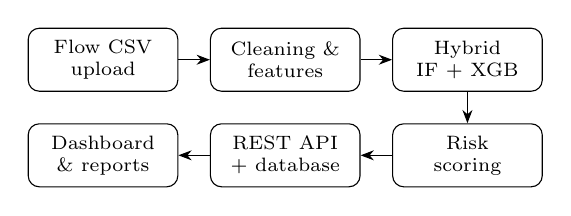
\begin{tikzpicture}[node distance=4mm, every node/.style={font=\scriptsize}, box/.style={draw, rounded corners, align=center, minimum width=1.9cm, minimum height=0.8cm}, >=Stealth]
\node[box] (a) {Flow CSV\\upload};
\node[box, right=of a] (b) {Cleaning \&\\features};
\node[box, right=of b] (c) {Hybrid\\IF + XGB};
\node[box, below=of c] (d) {Risk\\scoring};
\node[box, left=of d] (e) {REST API\\+ database};
\node[box, left=of e] (f) {Dashboard\\\& reports};
\draw[->] (a)--(b); \draw[->] (b)--(c); \draw[->] (c)--(d); \draw[->] (d)--(e); \draw[->] (e)--(f);
\end{tikzpicture}
\caption{Processing pipeline from uploaded flows to analyst-facing alerts.}
\label{fig:arch}
\end{figure}

\subsection{Cleaning and Feature Engineering}
Column names are trimmed, non-numeric columns dropped, infinite values converted to missing values, duplicate rows removed and rows without a label discarded. A preprocessor fitted on the training split only imputes medians, winsorises each feature at the 0.1th and 99.9th percentiles, applies a signed logarithm $\operatorname{sgn}(x)\log(1+|x|)$ and standardises. Derived features capture forward/backward packet and byte ratios, bytes per packet, packets per millisecond and the SYN-minus-ACK flag difference. Features correlated above 0.95 are pruned, and the 40 features with the highest mutual information with the label are kept.

Table~\ref{tab:prep} lists the stages in the order they run, and Table~\ref{tab:fe} lists the engineered features.

\begin{table}[!htb]
\caption{Preprocessing pipeline (fitted on training data only).}
\label{tab:prep}
\centering\footnotesize
\begin{tabular}{@{}cp{2.2cm}p{4.2cm}@{}}
\hline
Step & Stage & Operation \\
\hline
1 & Clean & trim headers, drop non-numeric columns, infinity to missing, remove duplicates and unlabeled rows \\
2 & Engineer & add ratio and rate features (Table~\ref{tab:fe}) \\
3 & Impute & replace missing values with training medians \\
4 & Winsorise & clip at 0.1th and 99.9th percentiles \\
5 & Transform & signed logarithm, then standardise \\
6 & Select & drop pairs correlated above 0.95; keep top 40 by mutual information \\
\hline
\end{tabular}
\end{table}

\begin{table}[!htb]
\caption{Engineered features.}
\label{tab:fe}
\centering\footnotesize
\begin{tabular}{@{}p{2.5cm}p{4.9cm}@{}}
\hline
Feature & Definition \\
\hline
pkt\_ratio\_fwd\_bwd & forward packets / (backward packets + 1) \\
total\_packets & forward + backward packets \\
byte\_ratio\_fwd\_bwd & forward bytes / (backward bytes + 1) \\
total\_bytes & forward + backward bytes \\
bytes\_per\_packet & total bytes / (total packets + 1) \\
pkts\_per\_ms & total packets / flow duration in ms \\
syn\_minus\_ack & SYN flag count $-$ ACK flag count \\
\hline
\end{tabular}
\end{table}

\subsection{Hybrid Scoring Model}
Let $x$ be a preprocessed flow. An Isolation Forest is fitted on benign training flows. Its raw anomaly score $r(x)$ is converted to an empirical percentile
\begin{equation}
s(x)=\frac{1}{|B|}\left|\{b\in B : r(b)\le r(x)\}\right|,
\end{equation}
where $B$ is a set of out-of-fold benign scores, so that $s(x)$ is approximately uniform for normal traffic and close to 1 for strong outliers. Out-of-fold scores are used for benign training rows to avoid the optimistic bias of scoring data the forest was fitted on.

The classifier $g$ is an XGBoost model trained on the augmented vector $[x, s(x)]$ after SMOTE balancing, yielding an attack probability $p(x)$. The final score is
\begin{equation}
f(x)=w\,p(x)+(1-w)\,s(x),\qquad w\in[0,1],
\end{equation}
and a flow is flagged when $f(x)\ge\tau$. The weight $w$ is chosen from a grid and $\tau$ from the precision--recall curve to maximise F1 on a validation set that contains one attack family never seen during training. This lets the blend learn how much to trust the anomaly branch when the classifier has no knowledge of the attack.

\subsection{Risk Scoring}
The score is mapped piecewise linearly so that $f=\tau$ gives a risk of 50, $f=0$ gives 0 and $f=1$ gives 100. Severity bands are Low ($<50$), Medium (50--69), High (70--89) and Critical ($\ge 90$). Flagged flows are labelled \emph{Known Attack} when $p\ge 0.5$, \emph{Zero-Day Attack} (suspected) when $p<0.5$ but the anomaly percentile is at least 0.95, and \emph{Suspicious Anomaly} otherwise. The reported confidence is the normalised distance from $\tau$; it measures decision margin and is not a calibrated probability. Fig.~\ref{fig:risk} plots the mapping for three example thresholds: because the mapping is anchored at $\tau$, a flow just above the learned decision boundary always lands at the start of the Medium band, whatever the absolute threshold.

\begin{figure}[!htb]
\centering
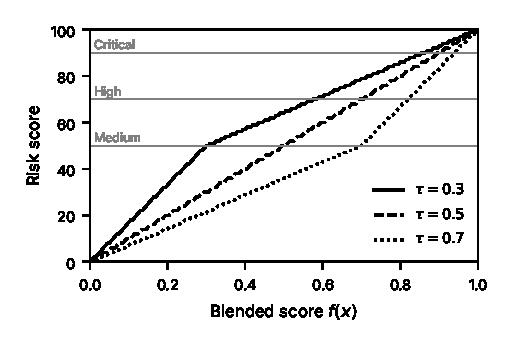
\includegraphics[width=0.85\columnwidth]{risk_mapping.pdf}
\caption{Risk score as a function of the blended score for example thresholds (generated from the system's risk-scoring function).}
\label{fig:risk}
\end{figure}

\begin{figure}[!htb]
\centering
\fbox{\begin{minipage}{0.93\columnwidth}\footnotesize
\textbf{Algorithm 1: Training the hybrid detector}\\[2pt]
\textbf{Input:} labelled flows $D$, held-out test family $F$\\
\textbf{Output:} model $(g,w,\tau)$ and risk mapping
\begin{enumerate}[leftmargin=1.2em,itemsep=0pt,topsep=2pt]
\item Remove $F$ from $D$; split benign and known attacks into train/validation; keep one known family $V$ for validation only.
\item Fit the preprocessor and feature selector on the training split.
\item Fit an Isolation Forest on benign training flows; compute out-of-fold benign scores and the percentile table.
\item Append $s(x)$ to each training vector; balance classes with SMOTE; fit XGBoost to obtain $p(x)$.
\item For each $w$ in a grid, compute $f$ on the validation set and choose $\tau$ maximising F1; keep the best $(w,\tau)$.
\item Refit the classifier on all training data plus $V$, keeping $(w,\tau)$.
\item Evaluate on benign test flows plus all flows of $F$.
\end{enumerate}
\end{minipage}}
\caption{Training and evaluation procedure.}
\label{fig:alg}
\end{figure}

\subsection{Model Configuration}
Table~\ref{tab:hp} gives the configuration of every model. All random seeds are fixed so that runs can be repeated.

\begin{table}[!htb]
\caption{Model hyper-parameters.}
\label{tab:hp}
\centering\footnotesize
\begin{tabular}{@{}p{1.75cm}p{5.6cm}@{}}
\hline
Model & Settings \\
\hline
Isolation Forest & 200 trees; scores calibrated on 3-fold out-of-fold benign scores \\
One-Class SVM & RBF kernel, $\gamma$ = scale, $\nu=0.05$, fitted on up to 4,000 benign flows \\
Random Forest & 200 trees \\
XGBoost & 300 trees, depth 6, learning rate 0.1, subsample 0.8, column sample 0.8; optional randomised search (8 draws, 3-fold, F1) over trees, depth, rate, subsample, column sample and minimum child weight \\
LightGBM & 300 trees, 63 leaves, learning rate 0.1, subsample 0.8, column sample 0.8 \\
SMOTE & 5 nearest neighbours, training split only \\
Hybrid & XGBoost as above on $[x,s(x)]$; $w$ from \{0, 0.1, \dots, 1\}; $\tau$ from PR curve \\
\hline
\end{tabular}
\end{table}

\begin{table}[!htb]
\caption{Risk bands and alert logic.}
\label{tab:risk}
\centering\footnotesize
\begin{tabular}{@{}p{0.9cm}p{1.2cm}p{5.2cm}@{}}
\hline
Risk & Severity & Threat type (if flagged) \\
\hline
0--49 & Low & Benign \\
50--69 & Medium & Suspicious Anomaly, or Known Attack if $p\ge0.5$ \\
70--100 & High, Critical (from 90) & Known Attack if $p\ge0.5$; Zero-Day (suspected) if $p<0.5$ and $s\ge0.95$; otherwise Suspicious Anomaly \\
\hline
\end{tabular}
\end{table}

\subsection{Computational Cost}
Isolation Forest training costs roughly $O(t\,\psi\log\psi)$ for $t$ trees built on sub-samples of size $\psi$, and scoring one flow costs $O(t\log\psi)$, independent of the training-set size. Histogram-based gradient boosting costs roughly $O(K\,n\,d)$ per run for $K$ trees, $n$ rows and $d$ features. Scoring is therefore linear in the number of uploaded flows, which is what allows a file of tens of thousands of flows to be analysed within a single web request. The out-of-fold calibration multiplies Isolation Forest training by the number of folds plus one, a one-off cost at training time.

\section{System Implementation}
The trained pipeline is served by a FastAPI process that accepts a CSV file and returns per-flow results. An ASP.NET Core~8 Web API authenticates users with ASP.NET Identity and JWT bearer tokens, enforces three roles (Admin, Analyst, Viewer), validates uploads, calls the inference service, and stores datasets, predictions, threats, risk scores, alerts, reports and audit logs in SQL Server through Entity Framework Core. An ASP.NET Core MVC front end built with Bootstrap and Chart.js presents totals, threat distribution, risk bands, detection trends and model metrics, and lets analysts acknowledge alerts and export PDF reports. Every upload, prediction, alert change and sign-in is written to an audit log.

\textbf{Analyst workflow.} A typical session has five steps: the analyst signs in and uploads a flow file; the server validates it and reports row counts, missing values and label distribution; the analyst starts an analysis, which sends the file to the inference service; the result page lists the highest-risk flows with their threat types and shows how risk is distributed across the file; and high-severity findings appear as open alerts that the analyst acknowledges or resolves, with each change recorded in the audit log. A threat or risk report for the analysis can then be exported as PDF for hand-over to other teams.

\textbf{Database.} Table~\ref{tab:db} lists the ten application tables. Deleting a dataset cascades to its flows, predictions, threats, risk scores and alerts; reports and audit entries survive deletion of their parent rows.

\begin{table}[!htb]
\caption{Database tables.}
\label{tab:db}
\centering\footnotesize
\begin{tabular}{@{}p{1.8cm}p{5.5cm}@{}}
\hline
Table & Purpose \\
\hline
Users, Roles & ASP.NET Identity accounts and roles \\
Datasets & uploaded file metadata, validation status and statistics \\
NetworkTraffic & sample of parsed flow fields per dataset \\
Predictions & one analysis run: totals, histogram, threshold, timing \\
RiskScores & per-flow risk, severity and confidence for flagged flows \\
Threats & flagged flows with type, severity and scores \\
Alerts & actionable alerts with Open, Acknowledged or Resolved status \\
Reports & stored threat and risk reports \\
AuditLogs & user, action, entity, time and address of each event \\
\hline
\end{tabular}
\end{table}

\begin{figure}[!htb]
\centering
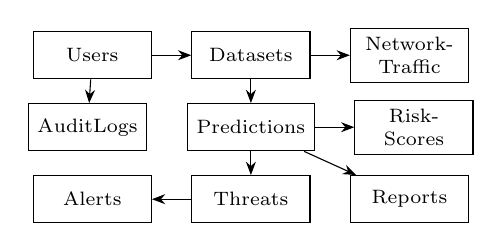
\begin{tikzpicture}[node distance=3mm and 5mm, every node/.style={font=\scriptsize}, ent/.style={draw, align=center, minimum width=1.5cm, minimum height=0.6cm}, >=Stealth]
\node[ent] (u) {Users};
\node[ent, right=of u] (d) {Datasets};
\node[ent, right=of d] (n) {Network-\\Traffic};
\node[ent, below=of d] (p) {Predictions};
\node[ent, left=of p] (a) {AuditLogs};
\node[ent, right=of p] (r) {Risk-\\Scores};
\node[ent, below=of p] (t) {Threats};
\node[ent, right=of t] (rp) {Reports};
\node[ent, left=of t] (al) {Alerts};
\draw[->] (u)--(d); \draw[->] (d)--(n); \draw[->] (d)--(p); \draw[->] (p)--(r); \draw[->] (p)--(t);
\draw[->] (t)--(al); \draw[->] (p)--(rp); \draw[->] (u)--(a);
\end{tikzpicture}
\caption{Simplified entity-relationship view; arrows point from parent to child. Users also own predictions, reports and alert acknowledgements.}
\label{fig:er}
\end{figure}

\textbf{Dashboard.} Table~\ref{tab:dash} describes the user-facing modules.

\begin{table}[!htb]
\caption{Web application modules.}
\label{tab:dash}
\centering\footnotesize
\begin{tabular}{@{}p{1.7cm}p{5.6cm}@{}}
\hline
Module & Content \\
\hline
Dashboard & total flows, threats, high-risk alerts, zero-day detections; charts for threat distribution, risk bands, detection trend and model metrics \\
Datasets & upload, validation message, row and column counts, label distribution, first rows \\
Detection & analyse a new file or a stored dataset; headline result, risk histogram, top threats \\
Threats, Alerts & filtered lists; acknowledge or resolve alerts \\
Reports & generate threat or risk report; PDF export \\
Admin & role assignment, account activation, audit log \\
\hline
\end{tabular}
\end{table}

The prediction endpoint returns, for the highest-risk flow, a compact record such as the following (the values shown illustrate the format only and are not experimental output):
\begin{figure}[h]
\centering
\fbox{\begin{minipage}{0.9\columnwidth}
\footnotesize\ttfamily \{ ``riskScore'': 96,\\
\hspace*{1em}``threatType'': ``Zero-Day Attack'',\\
\hspace*{1em}``severity'': ``Critical'',\\
\hspace*{1em}``confidence'': ``98\%'' \}
\end{minipage}}
\caption{Response format (illustrative values).}
\end{figure}

\textbf{Interfaces.} Table~\ref{tab:api} lists the main REST endpoints, and Table~\ref{tab:roles} shows what each role may do.

\begin{table}[!htb]
\caption{Main REST endpoints.}
\label{tab:api}
\centering\footnotesize
\begin{tabular}{@{}p{1.9cm}p{5.4cm}@{}}
\hline
Endpoint & Function \\
\hline
POST /register, /login & create account, obtain JWT \\
POST /upload & upload and validate a flow CSV \\
GET /datasets & list datasets, with preview and statistics routes \\
POST /predict & analyse a file or stored dataset; returns risk score, threat type, severity, confidence \\
GET /threats, /alerts & filtered lists; alert status can be updated \\
GET /reports & list reports; create and export as PDF \\
GET /audit-logs & administrator audit trail \\
\hline
\end{tabular}
\end{table}

\begin{table}[!htb]
\caption{Role permissions.}
\label{tab:roles}
\centering\footnotesize
\begin{tabular}{@{}lccc@{}}
\hline
Action & Admin & Analyst & Viewer \\
\hline
View dashboard, threats, alerts, reports & yes & yes & yes \\
Upload data, run predictions & yes & yes & no \\
Update alerts, create reports & yes & yes & no \\
Delete datasets, manage users, view audit log & yes & no & no \\
\hline
\end{tabular}
\end{table}

\textbf{Security.} Passwords are hashed by ASP.NET Identity and must contain eight characters with upper-case, lower-case and a digit; five failed sign-ins lock an account for fifteen minutes. Tokens are signed with a secret supplied through the environment. The inference service is reached with a shared key over a private network, uploads are limited in size and type, and password-reset requests return the same message whether or not an account exists.

\section{Experimental Setup}
\textbf{Environment.} Table~\ref{tab:env} lists the software stack.

\begin{table}[!htb]
\caption{Software environment.}
\label{tab:env}
\centering\footnotesize
\begin{tabular}{@{}p{2.2cm}p{5.1cm}@{}}
\hline
Layer & Technology \\
\hline
Machine learning & Python 3, scikit-learn, XGBoost, LightGBM, imbalanced-learn, pandas, NumPy \\
Inference service & FastAPI served by Uvicorn \\
Backend & ASP.NET Core 8 Web API, Entity Framework Core, ASP.NET Identity, JWT bearer authentication \\
Database & SQL Server \\
Front end & ASP.NET Core MVC, Bootstrap 5, Chart.js \\
Packaging & Docker, Docker Compose; Render blueprint for hosting \\
\hline
\end{tabular}
\end{table}

\begin{figure}[!htb]
\centering
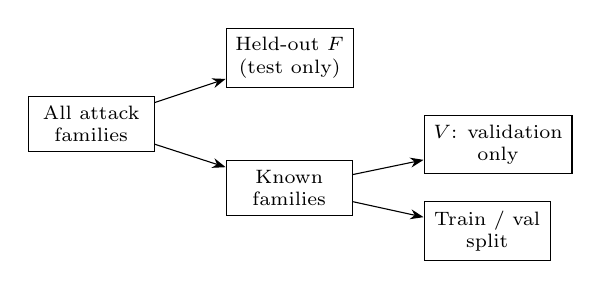
\begin{tikzpicture}[every node/.style={font=\scriptsize}, box/.style={draw, align=center, minimum height=0.7cm, minimum width=1.6cm}, >=Stealth]
\node[box] (all) {All attack\\families};
\node[box, above right=0.1cm and 0.9cm of all] (F) {Held-out $F$\\(test only)};
\node[box, below right=0.1cm and 0.9cm of all] (K) {Known\\families};
\node[box, right=0.9cm of K, yshift=0.55cm] (V) {$V$: validation\\only};
\node[box, right=0.9cm of K, yshift=-0.55cm] (T) {Train / val\\split};
\draw[->] (all)--(F); \draw[->] (all)--(K); \draw[->] (K)--(V); \draw[->] (K)--(T);
\end{tikzpicture}
\caption{How attack families are allocated in each experiment.}
\label{fig:proto}
\end{figure}

\textbf{Zero-day protocol.} For each attack family $F$, all flows of $F$ are removed from training and validation. Benign flows are split 60/20/20 into train, validation and test. Known attack families are split the same way, except that one of them is held out entirely as the pseudo-unknown validation family. The test set is the benign test portion plus every flow of $F$. Reported numbers are means over held-out families.

\textbf{Split and validation strategy.} Table~\ref{tab:split} shows how each family of flows is divided. Statistics for scaling and selection come from the training portion alone, so no information from validation or test flows reaches the preprocessing. Seeds are fixed, and the whole protocol can be repeated with different seeds to report variation.

\begin{table}[!htb]
\caption{Data partitions per held-out family $F$.}
\label{tab:split}
\centering\footnotesize
\begin{tabular}{@{}p{2.4cm}ccc@{}}
\hline
Traffic & Train & Validation & Test \\
\hline
Benign & 60\% & 20\% & 20\% \\
Known attack families & 60\% & 20\% & --- \\
Pseudo-unknown family $V$ & --- & 100\% & --- \\
Held-out family $F$ & --- & --- & 100\% \\
\hline
\end{tabular}
\end{table}

\textbf{Threshold optimisation.} For every model the decision threshold is the score at which F1 is highest on the validation precision--recall curve. The same rule is applied to the unsupervised and supervised models, so differences in the table come from the scores themselves rather than from a favourable default cut-off. Because the validation set contains an attack family that the classifier never saw, the chosen threshold reflects the situation the system faces at deployment.

\textbf{Planned ablations.} To show which design choice matters, the following variants will be evaluated under the same protocol (Table~\ref{tab:abl}).

\begin{table}[!htb]
\caption{Ablation variants and the question each answers.}
\label{tab:abl}
\centering\footnotesize
\begin{tabular}{@{}p{2.3cm}p{5.0cm}@{}}
\hline
Variant & Question \\
\hline
No anomaly feature & Does appending $s(x)$ help the classifier? \\
$w=1$ (classifier only) & How much does the blend add over the classifier alone? \\
$w=0$ (anomaly only) & How far does unsupervised scoring go by itself? \\
No SMOTE & Does balancing change recall on unseen families? \\
No engineered features & Do ratio and rate features add information? \\
No feature selection & Is the top-40 filter helping or hurting? \\
\hline
\end{tabular}
\end{table}

\textbf{Models.} Isolation Forest and One-Class SVM (trained on benign data only), Random Forest, XGBoost and LightGBM (trained on SMOTE-balanced data), and the proposed hybrid. Every model receives a decision threshold chosen by maximising F1 on the same validation set, so no model benefits from an untuned default.

\textbf{Metrics.} Accuracy, precision, recall, F1-score and error rate (one minus accuracy), together with false-positive rate, Matthews correlation coefficient, ROC-AUC and PR-AUC in the supplementary tables. XGBoost hyper-parameters are tuned by randomised search with three-fold cross-validation on F1.

With $TP$, $FP$, $TN$ and $FN$ denoting flagged attacks, false alarms, correct benign decisions and missed attacks,
\begin{align}
\text{Precision}&=\frac{TP}{TP+FP}, & \text{Recall}&=\frac{TP}{TP+FN},\\
\text{F1}&=\frac{2\,\text{Precision}\cdot\text{Recall}}{\text{Precision}+\text{Recall}}, & \text{Error}&=\frac{FP+FN}{TP+FP+TN+FN}.
\end{align}
Because a hidden attack family is usually a minority of the test set, accuracy alone can hide missed attacks; recall and F1 are therefore reported next to error rate.

\section{Deployment Architecture}
The system runs as three containers and one managed database (Table~\ref{tab:deploy}). The web application is the only component intended for end users; the API is also reachable for integration and exposes interactive documentation; the inference service is private and is called with a shared secret. Configuration, including connection strings, signing keys and the administrator account, is supplied through environment variables, never stored in the repository. Each public service exposes a health endpoint used by the host to restart failed instances, and uploaded files are kept on a persistent disk so that earlier datasets can be re-analysed after a redeployment.

\begin{table}[!htb]
\caption{Deployed components.}
\label{tab:deploy}
\centering\footnotesize
\begin{tabular}{@{}p{1.5cm}p{1.9cm}p{3.8cm}@{}}
\hline
Component & Exposure & Responsibility \\
\hline
Web & public & MVC pages, session cookie holding the user's token \\
API & public & authentication, validation, persistence, reports, calls the inference service \\
Inference & private & loads the trained bundle; scores uploaded flows \\
Database & private & SQL Server tables of Table~\ref{tab:db} \\
\hline
\end{tabular}
\end{table}

The trained model is stored as a single serialised bundle containing the preprocessor, feature selector, classifier, anomaly scorer, blend weight and threshold, so that inference applies exactly the transformations fitted at training time. Re-training produces a new bundle, and the service is restarted to load it. Because the bundle is a pickled object, it must come only from a trusted build process and never from user uploads.

\section{Verification Plan}
Table~\ref{tab:test} lists the verification activities. Only the first has been carried out at the time of writing, on generated data used purely to confirm that the pipeline runs end to end; no performance claim is drawn from it.

\begin{table}[!htb]
\caption{Verification activities and status.}
\label{tab:test}
\centering\footnotesize
\begin{tabular}{@{}p{3.3cm}p{2.2cm}p{1.6cm}@{}}
\hline
Activity & Scope & Status \\
\hline
Pipeline smoke test on generated flows & training, comparison, prediction, inference service & done \\
Zero-day experiments on real data & CIC-IDS2017, all families & pending \\
API endpoint tests & authentication, upload, predict, alerts, reports & pending \\
Role and access tests & permission matrix & pending \\
Large-file and malformed-CSV tests & upload validation & pending \\
Deployment health checks & web, API, inference service & pending \\
\hline
\end{tabular}
\end{table}

\section{Results and Discussion}
Table~\ref{tab:cmp} compares the six models under the zero-day protocol on CIC-IDS2017. The proposed hybrid has an error rate of \hybErr{}, accuracy \hybAcc{}, precision \hybPrec{}, recall \hybRec{} and F1-score \hybFscore{}. The strongest baseline by error rate is \bestBaseName{} at \bestBaseErr{}, giving a relative error change of \relRedBase{} for the hybrid. Against the error rate reported for the base paper, \paperErr{}, the relative change is \relRedPaper{}.

\begin{table}[!htb]
\caption{Zero-day comparison on CIC-IDS2017 (mean over held-out attack families; best value in bold).}
\label{tab:cmp}
\centering\footnotesize
\begin{tabular}{lccccc}
\hline
Model & Acc. & Prec. & Rec. & F1 & Err. \\
\hline
\multicolumn{6}{c}{[run results\_to\_latex.py after model\_compare.py]} \\
\hline
\end{tabular}

\end{table}

Table~\ref{tab:fam} breaks the error rate down by held-out family, which shows whether the hybrid helps uniformly or only on some attack types.

\begin{table}[!htb]
\caption{Error rate by held-out attack family on CIC-IDS2017 (best per column in bold).}
\label{tab:fam}
\centering\scriptsize
\resizebox{\columnwidth}{!}{\begin{tabular}{l}
\hline
[run results\_to\_latex.py after model\_compare.py] \\
\hline
\end{tabular}
}
\end{table}

% AFTER RUNNING THE EXPERIMENTS, add 1-2 paragraphs here that interpret YOUR table:
%  - which held-out families are easy/hard (use ML/results/cicids2017_per_family.csv)
%  - precision/recall trade-off of the unsupervised vs supervised models
%  - whether the hybrid beats the baselines; if not, say so and discuss why
% Do not write conclusions that the numbers do not support.

\textbf{Threats to validity.} Results depend on the label quality of CIC-IDS2017 \cite{engelen2021troubleshooting}; treating each attack family as ``unknown'' only approximates truly novel attacks, because families share protocol-level behaviour; and the comparison with the base paper is indicative only, since its evaluation protocol and data splits differ from ours.

\section{Limitations and Ethical Considerations}
The framework inherits the weaknesses of its parts. An Isolation Forest trained on one network's benign traffic will raise alarms on legitimate behaviour that network has never produced, so thresholds must be re-tuned when a deployment changes. Flow statistics do not see payloads, so attacks that look like ordinary flows can be missed. The ``zero-day'' label produced by the system means unrecognised and anomalous, not confirmed novel; a human analyst should review every alert before action. Uploaded traffic can reveal user behaviour, so datasets should be anonymised, access is restricted by role, and the audit log records who viewed or changed what. Finally, public benchmark traffic is synthetic or laboratory-generated, and performance on it does not guarantee performance on production networks.

\section{Conclusion and Future Work}
We presented a hybrid anomaly-and-classification framework for detecting unseen attack traffic, a risk-scoring layer for analysts, and a deployable web system around it. Under a leave-one-attack-family-out protocol the hybrid achieved an error rate of \hybErr{} versus \bestBaseErr{} for the best baseline. The accompanying source code, SQL scripts, container definitions and deployment guide allow the full system to be rebuilt from a clean checkout, and the experiment scripts regenerate every table in this paper directly from the saved result files. Future work includes cross-dataset evaluation on CTU-13 and USTC-TFC2016, online adaptation as traffic drifts, calibrated confidence estimates, explanations of which features drive a score, and evaluation on live captures.

\bibliographystyle{IEEEtran}
\bibliography{references}
\end{document}
